\begin{filecontents*}{references.bib}
@inproceedings{dragos2022angry,
  title={Angry or sad? emotion annotation for extremist content characterisation},
  author={Dragos, Valentina and Battistelli, Delphine and Etienne, Aline and Constable, Yol{\`e}ne},
  booktitle={Proceedings of the Thirteenth Language Resources and Evaluation Conference},
  pages={193--201},
  year={2022}
}

@phdthesis{etienne2023analyse,
  title={Analyse automatique des {\'e}motions dans les textes: contributions th{\'e}oriques et applicatives dans le cadre de l'{\'e}tude de la complexit{\'e} des textes pour enfants},
  author={Etienne, Aline},
  year={2023},
  school={Universit{\'e} de Nanterre-Paris X}
}

@inproceedings{dragos2023comparison,
  title={Comparison of Classification Techniques for Extremism Detection in French Social Media},
  author={Dragos, Valentina and Constable, Yol{\`e}ne},
  booktitle={2023 26th International Conference on Information Fusion (FUSION)},
  pages={1--6},
  year={2023},
  organization={IEEE}
}

@inproceedings{dragos2024exploring,
  title={Exploring the Emotional Dimension of French Online Toxic Content},
  author={Dragos, Valentina and Battistelli, Delphine and Sow, Fatou and Etienne, Aline},
  booktitle={Proceedings of the 2024 Joint International Conference on Computational Linguistics, Language Resources and Evaluation (LREC-COLING 2024)},
  pages={6945--6954},
  year={2024}
}

@misc{etienne2024emotionidentificationfrenchwritten,
  title={Emotion Identification for French in Written Texts: Considering their Modes of Expression as a Step Towards Text Complexity Analysis},
  author={Aline {\'E}tienne and Delphine Battistelli and Gw{\'e}nol{\'e} Lecorv{\'e}},
  year={2024},
  eprint={2405.14385},
  archivePrefix={arXiv},
  primaryClass={cs.CL},
  url={https://arxiv.org/abs/2405.14385}
}

@article{battistelli2025introduction,
  title={Introduction to the Special Issue of the TAL Journal on Abusive Language: Linguistic Resources, Methods and Applications},
  author={Battistelli, Delphine and Benamara, Farah and Patti, Viviana},
  journal={Traitement Automatique des Langues},
  volume={65},
  number={3},
  pages={7--20},
  year={2025}
}

@book{micheli2014,
  author    = {Micheli, Rapha{\"e}l},
  title     = {Les {\'e}motions dans les discours. Mod{\`e}le d'analyse, perspectives empiriques},
  publisher = {De Boeck Sup{\'e}rieur},
  address   = {Louvain-la-Neuve},
  series    = {Champs linguistiques},
  year      = {2014},
  doi       = {10.3917/dbu.mchel.2014.01}
}

@inproceedings{etienne2022,
  author    = {Etienne, Aline and Battistelli, Delphine and Lecorv{\'e}, Gw{\'e}nol{\'e}},
  title     = {A ({P}sycho-){L}inguistically Motivated Scheme for Annotating and Exploring Emotions in a Genre-Diverse Corpus},
  booktitle = {Proceedings of the Thirteenth Language Resources and Evaluation Conference},
  publisher = {European Language Resources Association},
  address   = {Marseille, France},
  month     = jun,
  year      = {2022},
  pages     = {603--612},
  url       = {https://aclanthology.org/2022.lrec-1.64/}
}

@article{battistelli2025,
  author  = {Battistelli, Delphine and {\'E}tienne, Aline},
  title   = {{ModalE}, une ressource lexicale de la modalit{\'e} au prisme des {\'e}motions},
  journal = {Les Carnets du Cediscor},
  number  = {35},
  year    = {2025},
  note    = {Num{\'e}ro : Marqueurs modaux, {\'e}nonciation et argumentation},
  url     = {https://hal.science/hal-05002259/document}
}
\end{filecontents*}

\documentclass{stageOnera}
%%
% Paquets
%

\usepackage[utf8]{inputenc}
\usepackage[T1]{fontenc}
\usepackage{csquotes}
\usepackage{url}
\usepackage{xcolor}
\definecolor{linkblue}{HTML}{2A8FBD}
\usepackage[
  colorlinks=true,
  linkcolor=linkblue,
  citecolor=linkblue,
  urlcolor=linkblue
]{hyperref}
\usepackage[numbers]{natbib}
\usepackage[french]{babel}
\usepackage{booktabs}
\usepackage{placeins}

%%
% Éléments du cartouche de titre
%

%%% Informations sur le stagiaire

%%%% Nom, prénom
\nom{Tsang}
\prenom{Gwendal}


%%%% Centre, département et unité
\departement{Palaiseau -- DTIS/MIDL}


%%% Informations sur le stage

%%%% Titre complet
% (utilier \par pour forcer le retour à la ligne)
\titre{Analyse automatique des émotions \par dans les contenus toxiques en ligne}

%%%% thématique (ICS, ISL, 3S, RA, ICIHS, PTI,MACS, IAD, COS)
\thematique{ICS}


%%%% Encadrant(s) (nom, prénom, département/unité)
% (utilier \par pour forcer le retour à la ligne)
\encadrantOnera{Delphine Battistelli \par Valentina Dragos}
\formation{Master 2 Traitement Automatique des Langues}

%%%% Mots clés (séparés par des virgules)
\motsCles{émotions, cyberharcèlement, toxicité en ligne, TAL, CamemBERT, EMOTYC}


\begin{document}

%% Création du cartouche de titre
\maketitle


%% Contenu
\section*{Objectifs}

L'objectif de ce stage est d'étudier dans quelle mesure les signaux émotionnels peuvent compléter l'analyse de contenus toxiques en ligne, en particulier dans des messages liés au cyberharcèlement adolescent. Le travail porte à la fois sur des ressources lexicales, des annotations linguistiques fines et l'évaluation d'un modèle neuronal existant de détection des émotions.




\section*{Contexte}

Le stage s'inscrit dans les travaux du service MIDL du DTIS sur l'analyse automatique des émotions dans les contenus toxiques et les situations de cyberharcèlement. Son point de départ théorique est un schéma d'annotation \citep{etienne2023analyse}. Ce schéma ne se limite pas à une liste de catégories émotionnelles : il décrit une \textit{Situation Émotionnelle} à partir d'un segment textuel, d'une catégorie émotionnelle, d'un mode d'expression, mais aussi d'éléments tels que l'expérienceur, la cause et la conséquence de l'émotion.\footnote{Le cadre théorique est résumé dans le fichier \href{https://github.com/GwenTsang/Eval-EMOTYC/blob/main/README.md}{README du dépôt Eval-EMOTYC}.}

Dans ce cadre, EMOTYC est à l'origine un processeur sémantique de la chaîne TextToKids : il extrait des descripteurs de complexité émotionnelle à partir d'un classifieur entraîné pour repérer, au niveau de la phrase, la présence d'une émotion, son mode d'expression, son type et sa catégorie.\footnote{Ressources publiques autour d'EMOTYC : site officiel de la chaîne TextToKids, \href{https://texttokids.ortolang.fr/}{texttokids.ortolang.fr} ; interface Hugging Face Space conçue pendant le stage pour utiliser EMOTYC au format ONNX, \href{https://huggingface.co/spaces/GwendalTsang/EMOTYC}{GwendalTsang/EMOTYC} ; backend TextToKids, \href{https://gitlab.huma-num.fr/texttokids/ttkwp3-2025}{ttkwp3-2025} ; poids du modèle au format \texttt{.bin}, \href{https://gitlab.huma-num.fr/texttokids/ttkwp3-2025/-/tree/main/text_complexity/server/src/resources/modele_emotyc/}{modele\_emotyc}.} La thèse d'Étienne présente ce processeur comme une traduction computationnelle du schéma d'annotation manuel, conçue pour l'analyse de textes destinés aux enfants et aux adolescents.

\begin{figure}[htbp]
  \centering
  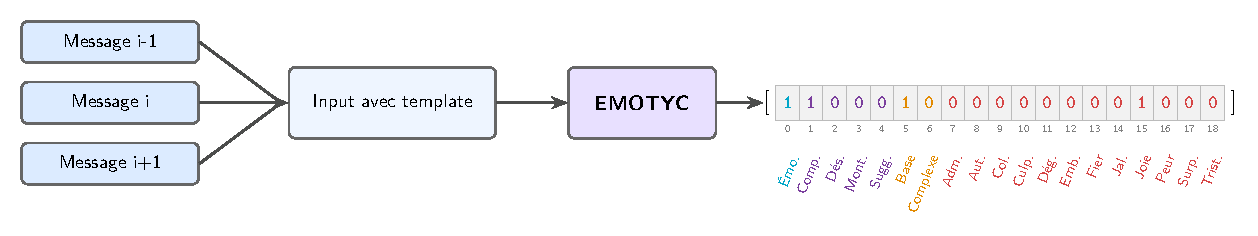
\includegraphics[width=\textwidth,height=0.25\textheight,keepaspectratio]{figures/schema.pdf}
  \caption{Schéma du modèle EMOTYC.}
  \label{fig:schema-emotyc}
\end{figure}

Une partie importante du stage a consisté à transposer ce schéma extrêmement fin à des messages de cyberagression adolescente. J'ai annoté manuellement 781 lignes issues d'un sous-ensemble de \textit{CyberAgression-Large} afin de produire un gold émotionnel \textit{CyberAggAdo} compatible avec les sorties d'EMOTYC.\footnote{Jeux de données exploités : \href{https://github.com/GwenTsang/EMOTYC/blob/master/data/CyberAdoAgg_gold_global_total_latest.xlsx}{CyberAdoAgg\_gold\_global\_total\_latest.xlsx}, \href{https://github.com/GwenTsang/Eval-EMOTYC/blob/main/golds/CyberAdoAgg_gold_global_total.xlsx}{CyberAdoAgg\_gold\_global\_total.xlsx}, sous-corpus CyberAggAdo par domaine dans \href{https://github.com/GwenTsang/Eval-EMOTYC/tree/main/golds/CyberAggAdo}{Eval-EMOTYC/golds/CyberAggAdo/}, échantillon \href{https://github.com/GwenTsang/Eval-EMOTYC/blob/main/golds/random_sample_120.xlsx}{random\_sample\_120.xlsx}, données TextToKids \href{https://github.com/GwenTsang/Eval-EMOTYC/blob/main/golds/TTK_test.parquet}{TTK\_test.parquet} et \href{https://github.com/GwenTsang/Eval-EMOTYC/blob/main/golds/emotexttokids_gold_flat.xlsx}{emotexttokids\_gold\_flat.xlsx}. Le corpus source CyberAgression-Large est disponible sur \href{https://github.com/aollagnier/CyberAgression-Large}{GitHub}.}

L'analyse automatique des émotions et de la toxicité en ligne (\textit{Abusive Language Detection}) se heurte à plusieurs difficultés. Les approches reposant uniquement sur une classification binaire décrivent imparfaitement la complexité linguistique et pragmatique des contenus, notamment lorsque la violence discursive s'exprime de manière implicite ou indirecte \citep{battistelli2025introduction}.

Cette limite est illustrée par Dragos et Constable~\citep{dragos2023comparison}, qui comparent différentes techniques de classification pour la détection de contenus extrémistes en français à partir d'un corpus de 1 728 textes. Leur étude confronte des modèles classiques, tels que les SVM associés à des représentations TF-IDF, Bag-of-Words ou à des traits linguistiques, à un modèle de langue pré-entraîné de type CamemBERT. Après rééquilibrage des données par SMOTE, CamemBERT obtient de bonnes performances, avec une exactitude de 0,78, une précision de 0,80, un rappel de 0,86 et une F-mesure de 0,79. Toutefois, un modèle plus classique, combinant SVM et TF-IDF, atteint des résultats comparables, voire supérieurs en rappel, avec une F-mesure de 0,83.

Ces résultats montrent que l'ajout de traits linguistiques de surface ne garantit pas une amélioration des performances : dans l'étude de Dragos et Constable~\citep{dragos2023comparison}, leur intégration au SVM entraîne au contraire une dégradation notable, la F-mesure chutant à 0,54. Les auteurs soulignent ainsi la difficulté à détecter l'extrémisme à partir de marqueurs génériques, en raison du caractère fuyant, contextuel et fortement subjectif de ce type de contenu. Cette limite justifie le recours à des marqueurs sémantiques plus profonds, parmi lesquels les émotions occupent une place centrale.


\section*{Objectifs scientifiques}

La modélisation automatique des émotions ne peut toutefois se réduire à l'identification de lexiques émotionnels explicites. Étienne~\citep{etienne2023analyse} montre les limites des approches fondées sur des ressources lexicales classiques et propose un schéma d'annotation distinguant quatre modes d'expression de l'émotion : le mode \textit{désigné}, lorsque l'émotion est exprimée par un lexique explicite ; le mode \textit{comportemental}, lorsqu'elle est associée à des manifestations physiques ou observables ; le mode \textit{montré}, lorsqu'elle apparaît à travers des indices syntaxiques, typographiques ou discursifs ; et le mode \textit{suggéré}, lorsqu'elle doit être inférée à partir du contexte socioculturel ou situationnel.

Les travaux de Dragos et al.~\citep{dragos2022angry} confirment la complexité d'un tel schéma lorsqu'il est appliqué à des contenus extrémistes. Dans leur étude consacrée à l'annotation émotionnelle de contenus extrémistes, les auteurs observent un accord satisfaisant pour l'identification des catégories émotionnelles, avec un rappel de 0,86, mais des performances beaucoup plus faibles pour la délimitation précise des déclencheurs linguistiques de l'émotion, avec une F-mesure de 0,54. Ce résultat met en évidence la difficulté à localiser précisément les indices émotionnels dans des discours où l'affect peut être diffus, implicite ou fortement dépendant du contexte.

Les objectifs scientifiques du stage consistent donc à dépasser une lecture strictement lexicale ou binaire des contenus toxiques, à examiner empiriquement le comportement de modèles d'analyse émotionnelle existants et à déterminer comment leurs sorties peuvent être interprétées pour caractériser plus finement des corpus issus des réseaux sociaux.


\section*{Démarche, déroulement et principaux résultats obtenus}

\subsection{Corpus, ressources et scripts mobilisés}

Le travail a combiné plusieurs types de ressources. D'une part, le corpus \textit{CyberAggAdo} a servi de terrain d'étude principal pour l'analyse de messages de cyberagression adolescente. D'autre part, les résultats sur \textit{TextToKids} ont fourni un point de comparaison avec le domaine d'entraînement d'EMOTYC. Les fichiers de référence, les scripts d'inférence et les sorties d'évaluation sont regroupés dans les dépôts associés au stage.\footnote{Scripts et sorties d'évaluation EMOTYC : \href{https://github.com/GwenTsang/Eval-EMOTYC/blob/main/orchestrate_emotyc_folder.py}{orchestrate\_emotyc\_folder.py}, \href{https://github.com/GwenTsang/Eval-EMOTYC/blob/main/emotyc_predict.py}{emotyc\_predict.py}, \href{https://github.com/GwenTsang/Eval-EMOTYC/blob/main/emotyc_predict_parquet.py}{emotyc\_predict\_parquet.py}, \href{https://github.com/GwenTsang/Eval-EMOTYC/blob/main/baseline_classifiers.py}{baseline\_classifiers.py}, rapport \href{https://github.com/GwenTsang/Eval-EMOTYC/blob/main/results/rapport_performances.md}{rapport\_performances.md}, résultats \href{https://github.com/GwenTsang/Eval-EMOTYC/tree/main/results/orchestrated_emotyc_CyberAggAdo}{orchestrated\_emotyc\_CyberAggAdo}, \href{https://github.com/GwenTsang/Eval-EMOTYC/tree/main/results/orchestrated_emotyc_subsets}{orchestrated\_emotyc\_subsets}, \href{https://github.com/GwenTsang/Eval-EMOTYC/tree/main/results/random_sample_120}{random\_sample\_120} et \href{https://github.com/GwenTsang/Eval-EMOTYC/tree/main/results/baselines}{baselines}.}

Un second volet a porté sur les marqueurs émotionnels et leur relation aux émotions et aux modes d'expression. Cette partie s'appuie sur la pipeline \textit{ExpressionEmotionnelle}, sur le corpus \textit{SimpleSitEmo} et sur les rapports statistiques produits à partir des annotations de \textit{CyberAggAdo}.\footnote{Ressources et scripts ExpressionEmotionnelle : \href{https://github.com/GwenTsang/ExpressionEmotionnelle/blob/main/data/SimpleSitEmo.parquet}{SimpleSitEmo.parquet}, \href{https://github.com/GwenTsang/ExpressionEmotionnelle/blob/main/data/SimpleSitEmo_xlsx.parquet}{SimpleSitEmo\_xlsx.parquet}, \href{https://github.com/GwenTsang/ExpressionEmotionnelle/blob/main/pipeline/run_analysis.py}{pipeline/run\_analysis.py}, \href{https://github.com/GwenTsang/ExpressionEmotionnelle/blob/main/pipeline/extract_markers.py}{extract\_markers.py}, \href{https://github.com/GwenTsang/ExpressionEmotionnelle/blob/main/pipeline/marker_specificity.py}{marker\_specificity.py}, \href{https://github.com/GwenTsang/ExpressionEmotionnelle/blob/main/pipeline/nlp_utils.py}{nlp\_utils.py}, \href{https://github.com/GwenTsang/ExpressionEmotionnelle/blob/main/tools/correlation.py}{tools/correlation.py}, \href{https://github.com/GwenTsang/ExpressionEmotionnelle/blob/main/results/hate_emotions_correlation_report.md}{hate\_emotions\_correlation\_report.md} et \href{https://github.com/GwenTsang/ExpressionEmotionnelle/blob/main/results/hate_modes_correlation_report.md}{hate\_modes\_correlation\_report.md}.}

\subsection{Annotations linguistiques fines et modèle EMOTION}

Le premier axe d'analyse a porté sur le module lexical \textit{EMOTION}. Ce module repose sur un lexique émotionnel qui associe des termes à des catégories.\footnote{Lexique et scripts associés : \href{https://github.com/GwenTsang/ExpressionEmotionnelle/blob/main/emotions/lexique_emotionnel.tsv}{lexique\_emotionnel.tsv}, \href{https://github.com/GwenTsang/ExpressionEmotionnelle/blob/main/tools/match_marker_values_to_lexicon.py}{match\_marker\_values\_to\_lexicon.py}, sorties de correspondance dans \href{https://github.com/GwenTsang/ExpressionEmotionnelle/tree/main/results/simplesitemo_lexicon_matching}{simplesitemo\_lexicon\_matching} et \href{https://github.com/GwenTsang/ExpressionEmotionnelle/tree/main/results/pipeline_2_compare_lexicon_matching}{pipeline\_2\_compare\_lexicon\_matching}.} Son principe est déterministe : après tokenisation, lemmatisation et filtrage de mots outils, chaque lemme est comparé aux entrées du lexique ; lorsqu'une entrée est trouvée, la catégorie correspondante est activée et les proportions de catégories sont calculées pour la séquence analysée. La lemmatisation est assurée par Stanza dans le module initial, tandis que les scripts de la pipeline permettent aussi de comparer des extractions avec spaCy.

Cette approche présente un intérêt méthodologique important : elle est interprétable, frugale et directement inspectable. Elle permet notamment d'examiner les catégories lexicales présentes dans les messages, par exemple les catégories liées au \textit{mépris}, au \textit{ressentiment}, à la \textit{colère} ou au \textit{dégoût}. Elle met aussi en évidence des limites attendues sur des messages adolescents : abréviations, fautes de frappe, graphies non standard, usages sarcastiques et variabilité contextuelle des termes émotionnels.

Un audit local du lexique et des marqueurs extraits a également permis d'identifier des points de normalisation utiles. Le lexique contient 1\,420 entrées, sans doublon apparent de terme, mais une variation de libellé entre \texttt{degout} et \texttt{dégoût} doit être harmonisée avant d'annoncer le nombre de catégories distinctes. Les scripts de comparaison entre marqueurs et lexique produisent des tableaux de correspondance et de propositions de réparation.

\subsection{Tests du modèle EMOTYC}

Le modèle EMOTYC a été développé dans le cadre du projet ANR TextToKids \citep{etienne2023analyse,etienne2024emotionidentificationfrenchwritten}.\footnote{Ressources externes : modèle \href{https://huggingface.co/TextToKids/CamemBERT-base-EmoTextToKids}{TextToKids/CamemBERT-base-EmoTextToKids} et publications du projet \href{https://texttokids.irisa.fr/publications/}{TextToKids}.} Il s'agit d'un modèle de type CamemBERT entraîné pour une classification multi-label : il prédit la présence d'une émotion, son niveau \textit{Base}/\textit{Complexe}, son mode d'expression et sa catégorie émotionnelle.

Les évaluations réalisées pendant le stage ont principalement repris la configuration contextuelle utilisée pour le modèle : la phrase cible est fournie avec son contexte immédiat, c'est-à-dire les phrases précédente et suivante. Les tableaux suivants synthétisent les performances obtenues avec un seuil de décision fixé à 0,5.

\begin{table}[htbp]
  \centering
  \small
  \begin{tabular}{lrrrr}
    \toprule
    Corpus & Exemples & Étiquettes & Macro-F1 & Micro-F1 \\
    \midrule
    \textit{TextToKids} & 27\,911 & 19 & 0,739 & 0,897 \\
    \textit{CyberAggAdo} global & 781 & 19 & 0,282 & 0,472 \\
    \bottomrule
  \end{tabular}
  \caption{Performances globales d'EMOTYC sur les deux corpus évalués.}
  \label{tab:perf-globales}
\end{table}

\begin{table}[htbp]
  \centering
  \scriptsize
  \setlength{\tabcolsep}{5pt}
  \begin{tabular}{lrrrrr}
    \toprule
    Étiquette & Support & Précision & Rappel & F1 & Kappa \\
    \midrule
    \multicolumn{6}{l}{\textit{Présence et niveau de complexité}} \\
    Émotion présente & 5\,374 & 0,927 & 0,933 & 0,930 & 0,914 \\
    Base & 4\,133 & 0,923 & 0,910 & 0,916 & 0,902 \\
    Complexe & 568 & 0,904 & 0,798 & 0,848 & 0,845 \\
    \addlinespace
    \multicolumn{6}{l}{\textit{Modes d'expression}} \\
    Comportementale & 1\,242 & 0,893 & 0,895 & 0,894 & 0,889 \\
    Désignée & 1\,499 & 0,925 & 0,929 & 0,927 & 0,923 \\
    Montrée & 971 & 0,900 & 0,872 & 0,886 & 0,882 \\
    Suggérée & 1\,909 & 0,833 & 0,800 & 0,816 & 0,803 \\
    \addlinespace
    \multicolumn{6}{l}{\textit{Catégories émotionnelles}} \\
    Admiration & 211 & 0,854 & 0,664 & 0,747 & 0,745 \\
    Autre & 1\,270 & 0,886 & 0,921 & 0,903 & 0,898 \\
    Colère & 1\,180 & 0,915 & 0,917 & 0,916 & 0,913 \\
    Culpabilité & 19 & 0,000 & 0,000 & 0,000 & 0,000 \\
    Dégoût & 52 & 1,000 & 0,077 & 0,143 & 0,143 \\
    Embarras & 162 & 0,818 & 0,778 & 0,798 & 0,796 \\
    Fierté & 202 & 0,840 & 0,777 & 0,807 & 0,806 \\
    Jalousie & 7 & 0,000 & 0,000 & 0,000 & 0,000 \\
    Joie & 888 & 0,912 & 0,853 & 0,881 & 0,878 \\
    Peur & 1\,047 & 0,894 & 0,886 & 0,890 & 0,886 \\
    Surprise & 824 & 0,913 & 0,886 & 0,899 & 0,896 \\
    Tristesse & 673 & 0,865 & 0,817 & 0,840 & 0,837 \\
    \bottomrule
  \end{tabular}
  \caption{Performances détaillées d'EMOTYC sur \textit{TextToKids} avec contexte. Le support correspond au nombre d'occurrences positives dans l'annotation de référence.}
  \label{tab:perf-texttokids}
\end{table}

\FloatBarrier

Sur \textit{TextToKids}, les performances sont élevées pour la présence d'une émotion, les modes d'expression et les catégories les plus représentées, avec une F1 supérieure à 0,88 pour la colère, la joie, la peur, la surprise, le mode \textit{désigné} et le mode \textit{comportemental}. Les résultats restent en revanche fragiles pour les classes très rares, comme la culpabilité, la jalousie ou le dégoût, où le support faible rend les scores instables malgré une exactitude globale élevée.

\FloatBarrier

\subsection*{Transposition aux réseaux sociaux}

La transposition d'un modèle tel qu'EMOTYC à des données issues des réseaux sociaux s'accompagne d'écarts de performance par rapport au domaine d'entraînement. Dragos et al.~\citep{dragos2024exploring} utilisent EMOTYC comme outil d'analyse automatique afin d'étudier la densité émotionnelle de corpus extrémistes, sexistes et haineux issus de Twitter et de forums. L'évaluation menée sur le corpus \textit{CyberAggAdo} global documente ces écarts dans des contextes discursifs plus bruités, plus courts et souvent plus implicites que ceux de son corpus d'entraînement.

\begin{table}[htbp]
  \centering
  \scriptsize
  \setlength{\tabcolsep}{5pt}
  \begin{tabular}{lrrrrr}
    \toprule
    Étiquette & Support & Précision & Rappel & F1 & Kappa \\
    \midrule
    \multicolumn{6}{l}{\textit{Présence et niveau de complexité}} \\
    Émotion présente & 398 & 0,620 & 0,706 & 0,660 & 0,258 \\
    Base & 363 & 0,633 & 0,485 & 0,549 & 0,245 \\
    Complexe & 14 & 0,212 & 0,500 & 0,298 & 0,280 \\
    \addlinespace
    \multicolumn{6}{l}{\textit{Modes d'expression}} \\
    Comportementale & 36 & 0,278 & 0,139 & 0,185 & 0,159 \\
    Désignée & 55 & 0,429 & 0,327 & 0,371 & 0,330 \\
    Montrée & 300 & 0,481 & 0,463 & 0,472 & 0,152 \\
    Suggérée & 54 & 0,158 & 0,056 & 0,082 & 0,048 \\
    \addlinespace
    \multicolumn{6}{l}{\textit{Catégories émotionnelles}} \\
    Admiration & 0 & 0,000 & 0,000 & 0,000 & -- \\
    Autre & 62 & 0,106 & 0,242 & 0,148 & 0,042 \\
    Colère & 289 & 0,492 & 0,429 & 0,458 & 0,173 \\
    Culpabilité & 3 & 0,000 & 0,000 & 0,000 & 0,000 \\
    Dégoût & 80 & 0,000 & 0,000 & 0,000 & 0,000 \\
    Embarras & 2 & 0,071 & 1,000 & 0,133 & 0,129 \\
    Fierté & 3 & 0,750 & 1,000 & 0,857 & 0,857 \\
    Jalousie & 6 & 0,000 & 0,000 & 0,000 & 0,000 \\
    Joie & 30 & 0,423 & 0,367 & 0,393 & 0,370 \\
    Peur & 4 & 0,154 & 0,500 & 0,235 & 0,229 \\
    Surprise & 5 & 0,333 & 0,400 & 0,364 & 0,359 \\
    Tristesse & 14 & 0,115 & 0,214 & 0,150 & 0,130 \\
    \bottomrule
  \end{tabular}
  \caption{Performances détaillées d'EMOTYC sur le corpus \textit{CyberAggAdo} global avec contexte. Le support correspond au nombre d'occurrences positives dans l'annotation de référence.}
  \label{tab:perf-cyberaggado}
\end{table}

\FloatBarrier

Les performances observées sur \textit{CyberAggAdo} sont nettement inférieures à celles obtenues sur \textit{TextToKids}. La présence d'une émotion reste la tâche la plus robuste, avec une F1 de 0,660, tandis que l'identification des modes d'expression et des catégories émotionnelles obtient des scores plus faibles : le mode \textit{suggéré} atteint 0,082 de F1 et la colère, très représentée dans le corpus, atteint 0,458 de F1. Ces écarts décrivent une sensibilité aux différences de domaine entre des textes jeunesse édités et des messages numériques conversationnels.\footnote{Analyses complémentaires et scripts associés : \href{https://github.com/GwenTsang/Eval-EMOTYC/blob/main/results/rapport_performances.md}{Eval-EMOTYC/results/rapport\_performances.md}, \href{https://github.com/GwenTsang/EMOTYC/blob/master/experimentations/error_analysis.py}{EMOTYC/experimentations/error\_analysis.py}, sorties \href{https://github.com/GwenTsang/EMOTYC/tree/master/experimentations/error_analysis_results}{error\_analysis\_results}, données structurées \href{https://github.com/GwenTsang/EMOTYC/tree/master/experimentations/error_analysis_results/structured}{error\_analysis\_results/structured}. Ces analyses relèvent notamment un exact match de 34,6~\% sur les 19 labels dans l'évaluation détaillée avec contexte, 80 occurrences gold de \textit{Dégoût} sans prédiction positive au seuil 0,5, ainsi que des incohérences structurelles entre labels d'émotion, de mode et de niveau.}

Dans ce contexte, l'extraction automatique des signaux émotionnels conserve un intérêt analytique. Dragos et al.~\citep{dragos2024exploring} montrent que la colère domine les corpus étudiés, mais que sa densité varie selon les types de contenus : elle représente 61,5~\% des émotions dans les textes haineux, contre 15,6~\% dans les contenus non haineux. À l'inverse, l'admiration apparaît davantage dans les contenus non haineux. Ces résultats indiquent que le profil émotionnel peut contribuer à caractériser les contenus toxiques et à compléter les approches strictement binaires de la toxicité en ligne \citep{dragos2024exploring,battistelli2025introduction}.

\subsection{Résultats descriptifs sur CyberAggAdo}

Les analyses statistiques réalisées sur les annotations de \textit{CyberAggAdo} indiquent que certaines émotions et certains modes sont associés au degré d'agressivité annoté.\footnote{Rapports et scripts correspondants : \href{https://github.com/GwenTsang/ExpressionEmotionnelle/blob/main/results/hate_emotions_correlation_report.md}{hate\_emotions\_correlation\_report.md}, \href{https://github.com/GwenTsang/ExpressionEmotionnelle/blob/main/results/hate_modes_correlation_report.md}{hate\_modes\_correlation\_report.md}, \href{https://github.com/GwenTsang/ExpressionEmotionnelle/blob/main/tools/correlation.py}{tools/correlation.py}, \href{https://github.com/GwenTsang/ExpressionEmotionnelle/blob/main/tools/prepare_correlation_dataset.py}{prepare\_correlation\_dataset.py}.} La colère et le dégoût sont plus fréquents dans les messages d'agressivité ouverte (\texttt{OAG}) que dans les messages non agressifs ou couverts. Le mode \textit{Montrée} est de son côté le mode le plus associé à l'agressivité ouverte.

Ces observations ne se substituent pas à une annotation manuelle ni à une évaluation de modèle. Elles fournissent plutôt un ensemble d'indices descriptifs permettant de relier les émotions, les modes d'expression, les rôles interactionnels et les catégories d'agressivité déjà présentes dans le corpus. Elles justifient l'intérêt d'articuler plusieurs niveaux d'analyse : lexique émotionnel, marqueurs linguistiques, annotations conversationnelles et sorties de modèles.


\section*{Perspectives}

Plusieurs prolongements peuvent être envisagés à partir des ressources produites. Une première piste consiste à mieux distinguer les configurations d'évaluation d'EMOTYC : avec ou sans contexte, seuil fixe ou seuil calibré, corpus continu ou échantillon non contigu. Cette distinction est importante car le contexte immédiat n'a pas le même statut dans un texte continu de \textit{TextToKids} et dans une conversation de cyberagression où les messages adjacents peuvent changer de locuteur, de cible ou d'intention.

Une deuxième piste consiste à appliquer un post-traitement logique aux sorties multi-labels. Lorsqu'une catégorie émotionnelle est prédite, le label global d'émotion devrait être cohérent avec cette prédiction ; de même, les labels \textit{Base} et \textit{Complexe} peuvent être dérivés des catégories émotionnelles plutôt que prédits indépendamment.

Une troisième piste concerne la normalisation contrôlée du langage numérique : abréviations, argot, allongements graphiques, fautes fréquentes et formes propres aux interactions adolescentes. Cette normalisation doit rester prudente, car certaines graphies non standard sont aussi des indices expressifs. Les scripts de \textit{ExpressionEmotionnelle} offrent un point de départ pour relier ces formes aux marqueurs émotionnels, au lexique et aux annotations de mode.

Enfin, les variables déjà présentes dans \textit{CyberAggAdo}, telles que \texttt{ROLE}, \texttt{TARGET}, \texttt{HATE}, \texttt{INTENTION} ou \texttt{SENTIMENT}, peuvent être utilisées comme variables d'analyse ou comme informations complémentaires dans de futures expériences. L'objectif serait de mieux décrire la relation entre émotion, agressivité, cible et position interactionnelle, sans réduire la détection du cyberharcèlement à une simple classification binaire.

%% Bibliographie
\bibliographystyle{onera}
\selectlanguage{french}
\bibliography{references}

\end{document}
